\documentclass[12pt,a4paper]{article}

\usepackage{graphicx}
\usepackage{abstract}
\usepackage{hyperref}
\usepackage{listings}
\usepackage{indentfirst}
\usepackage{amssymb}

\graphicspath{ {./images/} }
\renewcommand{\abstractname}{\large{Timestamps}}

\setlength{\parindent}{0.5in}

\title{Homework Template}
\author{Chris Nutter\thanks{Dedicated to @QuesoGrande a.k.a. Jared D.}}

% --> Here we go, satellite radio, y'all get hit with a...

\begin{document}

\maketitle

\begin{abstract}
    \noindent
    \begin{center}\textbf{Date + Time}\end{center}
        Don't forget to add two backslashes after you type out this statement. :) 
    
\end{abstract}

\tableofcontents    

% --> First Chapter

\section{Title}
    Lorem ipsum dolor sit amet, consectetur adipiscing elit, sed do eiusmod tempor incididunt ut labore et dolore magna aliqua. Ut enim ad minim veniam, quis nostrud exercitation ullamco laboris nisi ut aliquip ex ea commodo consequat. Duis aute irure dolor in reprehenderit in voluptate velit esse cillum dolore eu fugiat nulla pariatur. Excepteur sint occaecat cupidatat non proident, sunt in culpa qui officia deserunt mollit anim id est laborum.
    \begin{center}\line(1,0){250}\end{center}

% --> Next Chapter

\end{document} 

% Possibly Important LaTeX Functions %
% ================================== %

%   \begin{figure}[hbtp]
%       \centering
%       \fbox{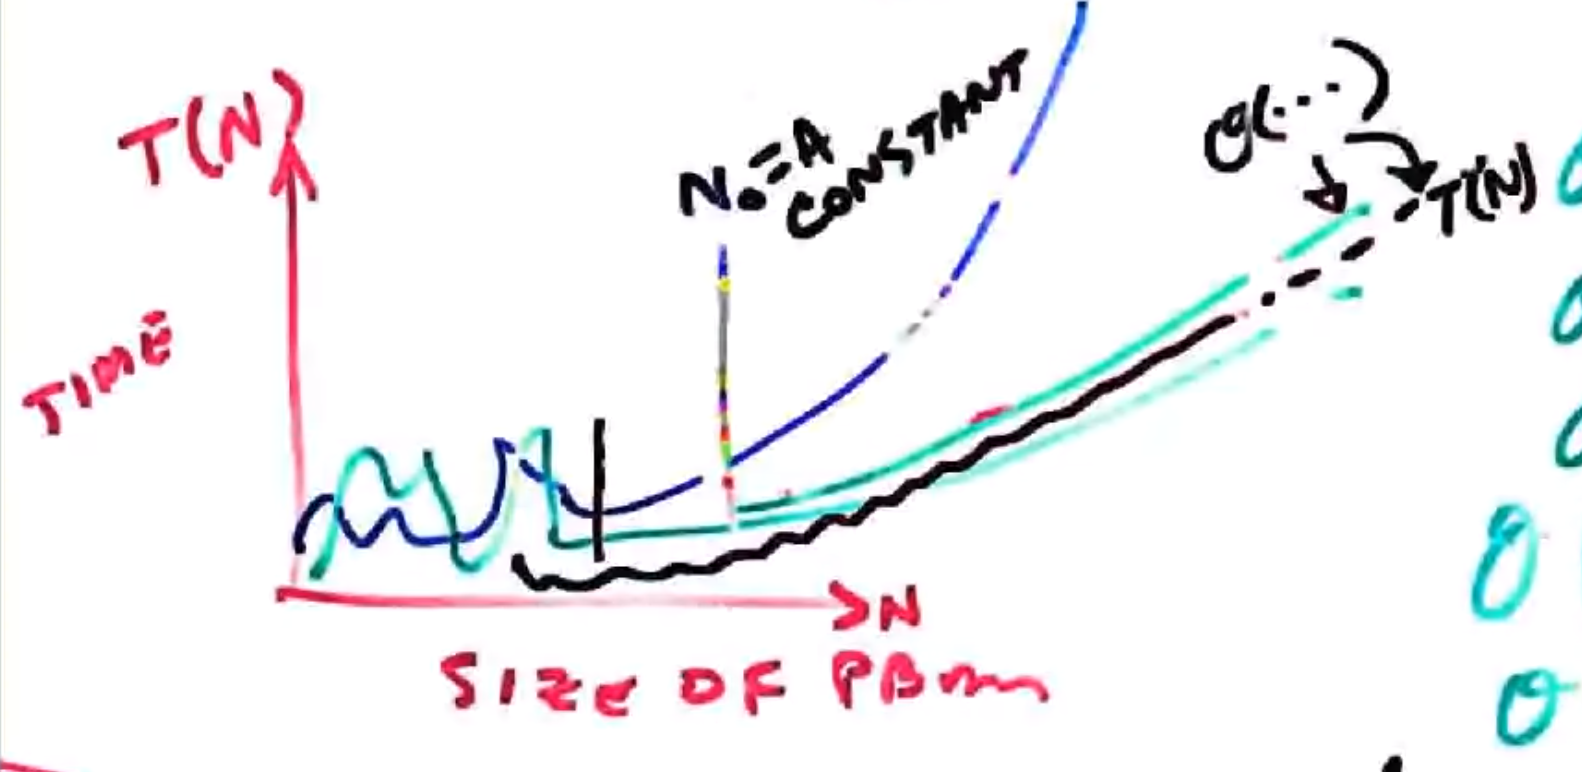
\includegraphics[width=13.8cm]{big_o.png}}
%       \caption{Big(O) Notation}
%   \end{figure}

%   \begin{lstlisting}[language=Python] 
%        print('hello world') 
%   \end{lstlisting}  

